\subsection{Análise de Requisitos}

\subsubsection{Atender e Registrar Pedidos dos Clientes}

O requisito de "Atender e Registrar Pedidos dos Clientes" é essencial para o funcionamento da transportadora, permitindo que os clientes façam pedidos e que essas solicitações sejam registradas no sistema. O ator envolvido é o cliente, que interage com o caso de uso "Receber Pedidos dos Clientes", enviando suas demandas por meio de um aplicativo ou plataforma online. O sistema, por sua vez, recebe esses pedidos, armazena as informações relevantes e os encaminha para processamento posterior. O registro adequado dos pedidos é crucial para a organização das demandas, possibilitando uma gestão mais eficiente das entregas e garantindo a satisfação dos clientes ao atender suas necessidades de forma precisa e oportuna.

\subsubsection{Permitir Ordens de Pedido dos Fornecedores}

O requisito de "Permitir Ordens de Pedido dos Fornecedores" busca assegurar o suprimento adequado de materiais e produtos essenciais para a operação da transportadora. Os fornecedores são os atores envolvidos, interagindo com o caso de uso "Emitir Ordens de Pedido aos Fornecedores". O sistema gera e envia eletronicamente as ordens de pedido, estabelecendo formalmente a solicitação de compra. A emissão de ordens de pedido é uma etapa crítica no controle da cadeia de suprimentos, permitindo que a transportadora mantenha um histórico organizado de suas transações comerciais com os fornecedores, garantindo a disponibilidade dos materiais e evitando problemas de estoque.

\subsubsection{Cadastrar Fornecedores}

O requisito de "Cadastrar Fornecedores" visa permitir que a transportadora mantenha um registro detalhado e atualizado das informações de seus fornecedores. O ator envolvido é o funcionário, que interage com o caso de uso "Cadastrar Fornecedores" para inserir os dados dos fornecedores no sistema. O cadastro organizado dos fornecedores é crucial para uma gestão eficiente da cadeia de suprimentos, permitindo à transportadora ter acesso rápido e fácil às informações relevantes sobre seus parceiros de negócios, facilitando a comunicação e a negociação com essas entidades.

\subsubsection{Gerenciar Estoques}

O requisito de "Gerenciar Estoques" é essencial para garantir o adequado controle dos níveis de estoque da transportadora. O ator envolvido é o funcionário, que interage com o caso de uso "Atualizar Estoques", responsável por ajustar as quantidades de estoque com base nas movimentações de entrada e saída de mercadorias. O gerenciamento eficiente dos estoques é crucial para evitar faltas ou excessos, permitindo que a transportadora mantenha uma quantidade adequada de produtos disponíveis para atender a demanda dos clientes de forma ágil e eficaz.

\subsubsection{Auxiliar na Tomada de Decisões Logísticas}

O requisito de "Auxiliar na Tomada de Decisões Logísticas" tem como objetivo fornecer informações relevantes para apoiar as decisões estratégicas e operacionais relacionadas à logística da transportadora. O ator envolvido é o funcionário, que interage com o caso de uso "Tomar Decisões Logísticas", que disponibiliza relatórios e dados relevantes para apoiar a tomada de decisões logísticas. A disponibilidade de informações precisas e atualizadas é essencial para a eficiência das operações logísticas, permitindo que a transportadora identifique oportunidades de otimização e reduza custos operacionais.

\subsubsection{Integrar Multi CD’s}

O requisito de "Integrar Multi CD’s" busca integrar os diversos Centros de Distribuição (CDs) da transportadora para coordenar e utilizar eficientemente os recursos disponíveis em diferentes locais. O ator envolvido é o Sistema de Roteirização, interagindo com os casos de uso "Verificar Capacidade do CD" e "Verificar Disponibilidade de Frota" para garantir a coordenação adequada das operações. A integração entre os CDs é crucial para a otimização da distribuição de produtos, permitindo que a transportadora acomode entregas de forma mais eficiente e reduza custos logísticos.

\subsubsection{Emitir Notas Fiscais}

O requisito de "Emitir Notas Fiscais" tem o propósito de documentar as transações comerciais realizadas pela

 transportadora. O ator envolvido é o funcionário, que interage com o caso de uso "Emitir Notas Fiscais", gerando os documentos fiscais para as transações realizadas. A emissão de notas fiscais é essencial para a conformidade legal e contábil da transportadora, garantindo a correta tributação das operações e o cumprimento das obrigações fiscais.

\subsubsection{Emitir Relatórios de Capacidade e Operação}

O requisito de "Emitir Relatórios de Capacidade e Operação" busca fornecer relatórios detalhados sobre a capacidade dos recursos da transportadora e o desempenho das operações. O ator envolvido é o Sistema de Roteirização, interagindo com o caso de uso "Emitir Relatórios de Utilização e de Operação", que gera os relatórios necessários para apresentar informações relevantes sobre a capacidade e o desempenho da operação logística. A disponibilidade desses relatórios é crucial para uma gestão eficiente da transportadora, permitindo que a empresa acompanhe o desempenho e identifique oportunidades de melhoria.

\subsubsection{Controlar os Indicadores Financeiros da Empresa}

O requisito de "Controlar os Indicadores Financeiros da Empresa" visa calcular e monitorar os indicadores financeiros relevantes para a transportadora. O ator envolvido é o Sistema Financeiro, que interage com o caso de uso "Calcular Indicadores", responsável por realizar os cálculos financeiros necessários. O controle adequado dos indicadores financeiros é essencial para a saúde financeira da transportadora, permitindo que a empresa tome decisões informadas e estratégicas para garantir a sustentabilidade e o crescimento do negócio.

\subsubsection{Armazenar Dados sobre a Frota de Caminhões}

O requisito de "Armazenar Dados sobre a Frota de Caminhões" tem o objetivo de manter um registro organizado dos dados da frota de caminhões da transportadora. O ator envolvido é o funcionário, que interage com o caso de uso "Cadastrar Funcionários e Administradores", onde também são inseridos os dados dos motoristas e da frota de caminhões. O armazenamento detalhado dos dados da frota é essencial para a gestão eficiente dos recursos e para garantir a manutenção adequada dos veículos, assegurando a disponibilidade e a confiabilidade dos caminhões para as operações de entrega.

\subsubsection{Permitir Avaliação Pelos Clientes}

O requisito de "Permitir Avaliação Pelos Clientes" tem o objetivo de permitir que os clientes avaliem os serviços prestados pela transportadora. O ator envolvido é o cliente, que interage com o caso de uso "Avaliar Serviço", fornecendo suas avaliações sobre o serviço recebido. A possibilidade de avaliação é fundamental para a satisfação dos clientes, permitindo que a transportadora obtenha feedback sobre a qualidade dos serviços e identifique oportunidades de melhoria para aprimorar a experiência do cliente.

\subsubsection{Permitir que o Cliente Acompanhe o Produto}

O requisito de "Permitir que o Cliente Acompanhe o Produto" visa oferecer aos clientes a possibilidade de acompanhar o status de suas entregas em tempo real. O ator envolvido é o cliente, que interage com o caso de uso "Acompanhar a Entrega", permitindo-lhes verificar o andamento das entregas e receber atualizações sobre o status de seus pedidos. Essa funcionalidade é essencial para aumentar a transparência e a confiança dos clientes na transportadora, proporcionando uma experiência de entrega mais satisfatória e garantindo que os clientes se sintam informados e envolvidos durante todo o processo.

\subsection{Diagrama de Caso de Uso (DCU)}

O Diagrama de Caso de Uso é uma poderosa ferramenta utilizada na Engenharia de Requisitos e no processo de análise e modelagem de sistemas de software. Essa representação gráfica tem como objetivo descrever de forma clara e detalhada as interações entre os atores e o sistema em questão, além de mapear as principais funcionalidades que o sistema oferece.

No contexto do projeto proposto para a transportadora, o Diagrama de Caso de Uso desempenha um papel estratégico na comunicação com os stakeholders, na identificação dos atores envolvidos e na definição clara das funcionalidades essenciais para atender às necessidades dos usuários. Essa representação visual permite uma compreensão comum entre a equipe de desenvolvimento, gerentes, clientes e outras partes interessadas, alinhando expectativas e objetivos desde o início do projeto. Por isso, segue o Diagrama de Caso de Uso proposto para a transportadora na figura \ref{fig:DCU}:

\begin{figure}[H]
    \centering
    \caption{Diagrama de Caso de Uso}
    \label{fig:DCU}
    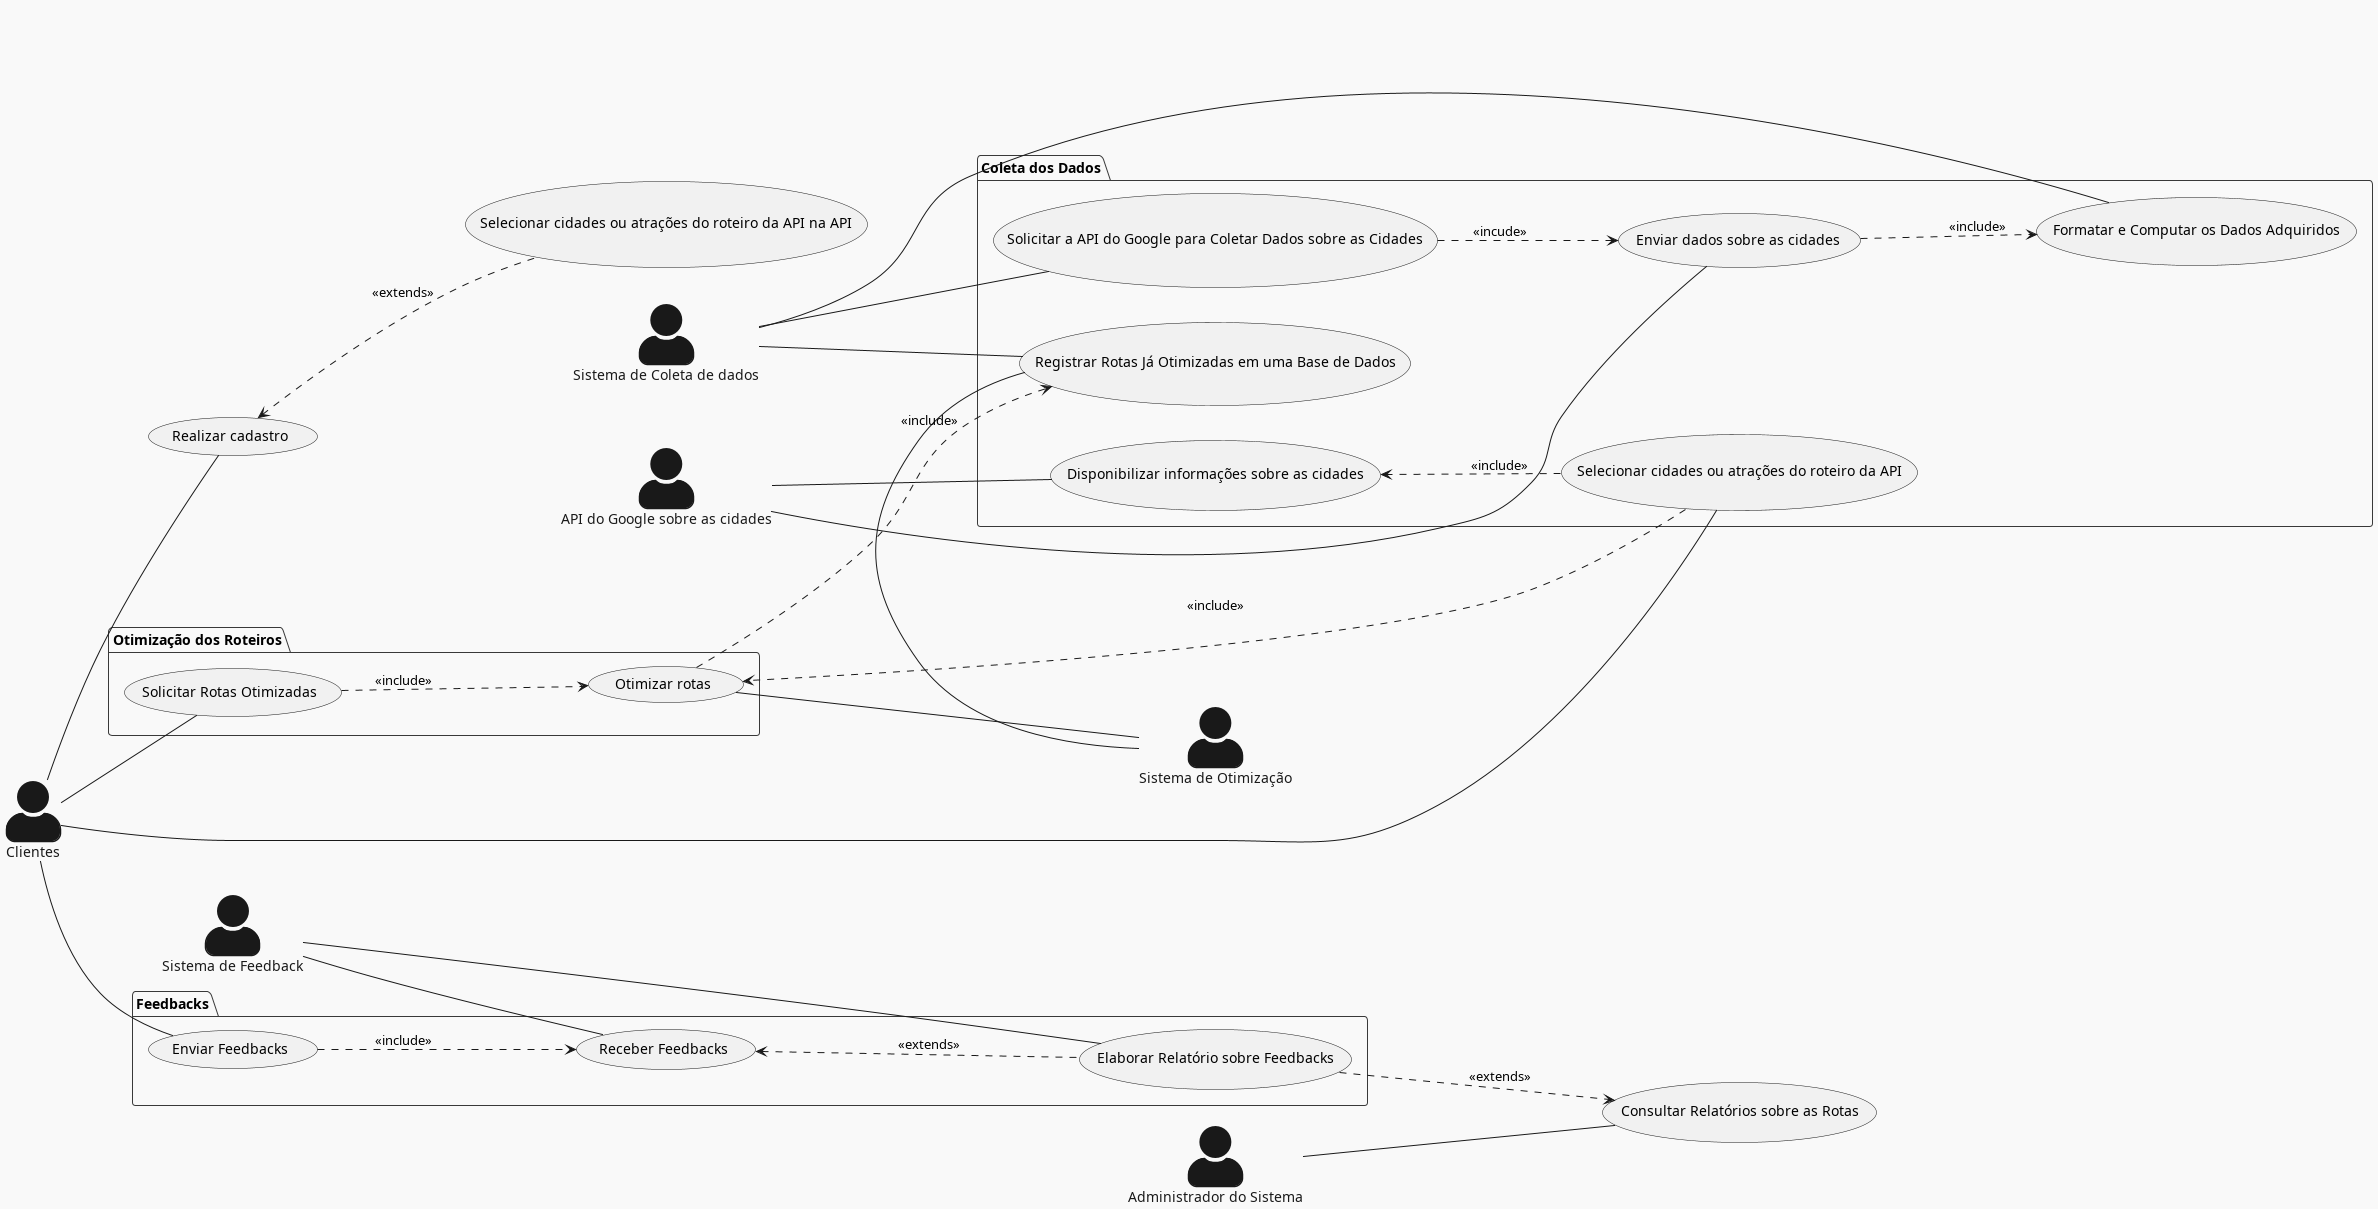
\includegraphics[scale=0.29]{Diagramas/DCU.png}\\
    \caption*{Fonte: Elaborado pelos autores}
\end{figure}

O Diagrama de Caso de Uso apresentado é uma representação visual que descreve de forma detalhada as interações entre os atores e o sistema proposto para a transportadora, oferecendo uma visão abrangente das funcionalidades do sistema e como elas se relacionam com os usuários e demais atores envolvidos.

Os atores no diagrama são representados por ícones distintos, como "Clientes", "Administrador do Sistema", "Funcionários", "Fornecedores", "Motoristas", "Sistema de Pagamentos", "Sistema de Roteirização" e "Sistema Financeiro". Cada ator representa uma entidade externa ao sistema e desempenha um papel específico na interação com o sistema.

As funcionalidades do sistema são representadas pelos casos de uso, que são elipses no diagrama. Cada caso de uso descreve uma ação ou funcionalidade que o sistema oferece e é identificado por um nome significativo. Os casos de uso são conectados aos atores relevantes por meio de linhas, mostrando as interações e comunicações entre os atores e o sistema.

Por exemplo, o caso de uso "Receber Pedidos dos Clientes" é conectado ao ator "Clientes", indicando que os clientes interagem com o sistema para registrar seus pedidos. Isso pode envolver a utilização de um aplicativo ou plataforma online em que os clientes preencham os detalhes do pedido, como produtos desejados, endereço de entrega e informações de pagamento.

Além disso, o diagrama também mostra as relações de inclusão e extensão entre os casos de uso. A relação de inclusão é representada por uma seta pontilhada e indica que um caso de uso inclui outro caso de uso. Por exemplo, o caso de uso "Calcular Rota Otimizada" está incluído em "Confirmar Pedido", o que significa que o cálculo da rota otimizada é uma etapa essencial no processo de confirmação do pedido.

A relação de extensão é representada por uma seta tracejada e indica que um caso de uso estende outro caso de uso, ou seja, adiciona funcionalidades opcionais. Por exemplo, o caso de uso "Emitir Relatórios de Utilização e de Operação" estende o caso de uso "Registrar Histórico de Entregas", o que significa que, após o registro do histórico de entregas, o sistema pode fornecer a opção de gerar relatórios adicionais para análise e controle da operação.
